\documentclass[aspectratio=169]{beamer}

% Tema y esquema de colores
\usetheme{Madrid}
\usecolortheme{dolphin}

% Paquetes esenciales
\usepackage[utf8]{inputenc}
\usepackage{amsmath}
\usepackage{graphicx}
\usepackage{listings}
\usepackage{tikz}
\usepackage{xcolor}
\usetikzlibrary{arrows,shapes,positioning,decorations.pathreplacing}

% Configuración para los bloques de código
\lstset{
  basicstyle=\ttfamily\small,
  keywordstyle=\color{blue},
  commentstyle=\color{green!50!black},
  stringstyle=\color{red},
  breaklines=true,
  showstringspaces=false,
  frame=single
}

\title{Fundamentos de la Generación de Números Aleatorios}
\subtitle{Estadística Computacional}
\author{Fred Torres Cruz}
\date{\today}

\begin{document}

\begin{frame}
    \titlepage
\end{frame}

\begin{frame}{Contenido}
    \tableofcontents
\end{frame}

\section{Introducción a la Generación de Números Aleatorios}

\begin{frame}{¿Qué son los números aleatorios?}
    \begin{block}{Definición}
        Un número aleatorio es una realización de una variable aleatoria que sigue una distribución de probabilidad específica.
    \end{block}
    
    \bigskip
    
    \begin{alertblock}{Conceptos clave}
        \begin{itemize}
            \item Los \textbf{números aleatorios verdaderos} provienen de fenómenos físicos.
            \item Los \textbf{números pseudoaleatorios} son secuencias generadas por algoritmos.
            \item En la práctica computacional, usamos generadores de números pseudoaleatorios (PRNG).
        \end{itemize}
    \end{alertblock}
\end{frame}

\begin{frame}{Aplicaciones de los números aleatorios}
    \begin{columns}
        \column{0.5\textwidth}
        \begin{itemize}
            \item Simulación estocástica
            \item Métodos de Monte Carlo
            \item Criptografía
            \item Muestreo aleatorio
            \item Algoritmos probabilísticos
        \end{itemize}
        
        \column{0.5\textwidth}
        \begin{tikzpicture}[scale=0.7]
            \draw[thick] (0,0) circle (2cm);
            \draw[thick] (-2,-2) rectangle (2,2);
            \foreach \i in {1,...,30} {
                \pgfmathsetmacro{\x}{2*rand()-1}
                \pgfmathsetmacro{\y}{2*rand()-1}
                \fill[blue] (2*\x,2*\y) circle (0.05cm);
            }
        \end{tikzpicture}
        \centering
        \tiny Aproximación de $\pi$ con Monte Carlo
    \end{columns}
\end{frame}

\section{Generadores Pseudoaleatorios}

\begin{frame}{Propiedades deseables en un PRNG}
    \begin{exampleblock}{Características principales}
        \begin{itemize}
            \item \textbf{Uniformidad}: distribución uniforme en el intervalo [0,1)
            \item \textbf{Independencia}: sin correlación entre números consecutivos
            \item \textbf{Período largo}: larga secuencia antes de repetirse
            \item \textbf{Reproducibilidad}: resultados reproducibles con la misma semilla
            \item \textbf{Eficiencia}: generación rápida con pocos recursos
            \item \textbf{Portabilidad}: resultados idénticos en distintas plataformas
        \end{itemize}
    \end{exampleblock}
\end{frame}

\begin{frame}{Generadores Congruenciales Lineales (LCG)}
    \begin{block}{Definición}
        Un generador congruencial lineal produce una secuencia de números enteros usando la fórmula recursiva:
        \begin{align}
        X_{n+1} &= (aX_n + c) \bmod m \\
        U_{n+1} &= X_{n+1}/m
        \end{align}
        donde:
        \begin{itemize}
            \item $a$ es el multiplicador
            \item $c$ es el incremento
            \item $m$ es el módulo
            \item $X_0$ es la semilla inicial
        \end{itemize}
    \end{block}
\end{frame}

\begin{frame}{Visualización de un LCG}
    \begin{tikzpicture}[scale=0.055]
        % Parámetros del LCG: X_{n+1} = (7X_n + 0) mod 53
        \draw[->] (0,0) -- (55,0) node[right] {$X_n$};
        \draw[->] (0,0) -- (0,55) node[above] {$X_{n+1}$};
        
        % Dibujar puntos para cada par (X_n, X_{n+1})
        \foreach \x [count=\i from 0] in {16,6,42,24,9,10,17,13,38,0,0,...} {
            \pgfmathsetmacro{\nextx}{mod(7*\x, 53)}
            \ifnum\i<10
                \fill[blue] (\x,\nextx) circle (1);
                \node[font=\tiny] at (\x,\nextx+2) {\i};
            \fi
        }
        
        % Línea diagonal para referencia
        \draw[dashed] (0,0) -- (53,53);
        
        % Etiquetas
        \node[below] at (25,0) {$a=7$, $c=0$, $m=53$, $X_0=16$};
    \end{tikzpicture}
    \caption{Secuencia de un LCG simple visualizada como pares $(X_n, X_{n+1})$}
\end{frame}

\begin{frame}{Problemas de los LCG}
    \begin{columns}
        \column{0.6\textwidth}
        \begin{alertblock}{Limitaciones}
            \begin{itemize}
                \item Período limitado por $m$
                \item Estructura de retícula en dimensiones altas
                \item Correlación entre valores sucesivos
            \end{itemize}
        \end{alertblock}
        
        \column{0.4\textwidth}
        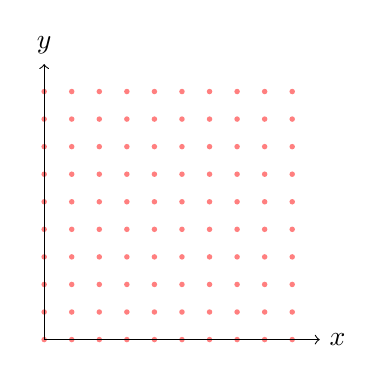
\begin{tikzpicture}[scale=0.35]
            % Estructura de retícula en 2D para un mal LCG
            \foreach \i in {0,...,9} {
                \foreach \j in {0,...,9} {
                    \fill[red, opacity=0.5] (\i,\j) circle (0.1);
                }
            }
            \draw[->] (0,0) -- (10,0) node[right] {$x$};
            \draw[->] (0,0) -- (0,10) node[above] {$y$};
        \end{tikzpicture}
        \tiny Estructura de retícula en 2D
    \end{columns}
\end{frame}

\begin{frame}{Implementación de un LCG básico en R}
    \begin{lstlisting}[language=R]
# Implementación simple de un generador LCG
lcg <- function(n, seed=123, a=1664525, c=1013904223, m=2^32) {
  x <- numeric(n)
  x[1] <- seed
  
  # Generar secuencia
  for (i in 2:n) {
    x[i] <- (a * x[i-1] + c) %% m
  }
  
  # Normalizar a [0,1)
  return(x/m)
}

# Generar 1000 números aleatorios
random_nums <- lcg(1000)

# Visualizar histograma
hist(random_nums, breaks=30, main="Histograma LCG",
     xlab="Valor", col="lightblue")
    \end{lstlisting}
\end{frame}

\begin{frame}{Implementación de un LCG básico en Python}
    \begin{lstlisting}[language=Python]
import numpy as np
import matplotlib.pyplot as plt

def lcg(n, seed=123, a=1664525, c=1013904223, m=2**32):
    """Implementación simple de un generador LCG"""
    x = np.zeros(n)
    x[0] = seed
    
    # Generar secuencia
    for i in range(1, n):
        x[i] = (a * x[i-1] + c) % m
    
    # Normalizar a [0,1)
    return x / m

# Generar 1000 números aleatorios
random_nums = lcg(1000)

# Visualizar histograma
plt.hist(random_nums, bins=30, color='skyblue', edgecolor='black')
plt.title('Histograma LCG')
plt.xlabel('Valor')
plt.ylabel('Frecuencia')
plt.show()
    \end{lstlisting}
\end{frame}

\section{Generador Mersenne Twister}

\begin{frame}{Generador Mersenne Twister}
    \begin{block}{Características principales}
        \begin{itemize}
            \item Desarrollado por Matsumoto y Nishimura (1998)
            \item Período extremadamente largo: $2^{19937}-1$
            \item Equidistribución en 623 dimensiones
            \item Pasa la mayoría de pruebas estadísticas
            \item Implementado por defecto en R, Python, C++, etc.
        \end{itemize}
    \end{block}
    
    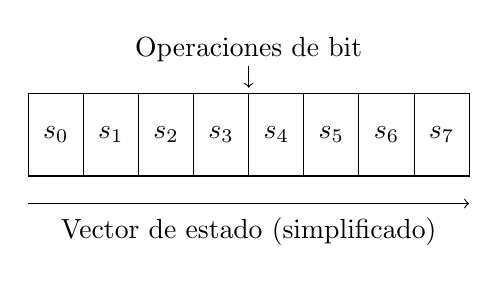
\begin{tikzpicture}[scale=0.7]
        % Representación simplificada del funcionamiento de MT
        \draw (0,0) rectangle (8,1.5);
        \foreach \x in {1,...,7} {
            \draw (\x,0) -- (\x,1.5);
        }
        
        \foreach \x [count=\i from 0] in {0,...,7} {
            \node at (\x+0.5,0.75) {$s_{\i}$};
        }
        
        \draw[->] (4,2) -- (4,1.6);
        \node at (4,2.3) {Operaciones de bit};
        
        \draw[->] (0,-0.5) -- (8,-0.5);
        \node at (4,-1) {Vector de estado (simplificado)};
    \end{tikzpicture}
\end{frame}

\begin{frame}{Funcionamiento de Mersenne Twister}
    \begin{columns}
        \column{0.6\textwidth}
        El algoritmo mantiene:
        \begin{itemize}
            \item Un vector de estado de 624 números de 32 bits
            \item Aplicación de operaciones bit a bit entre elementos
            \item Transformación adicional ("tempering") antes de retornar
        \end{itemize}
        
        \column{0.4\textwidth}
        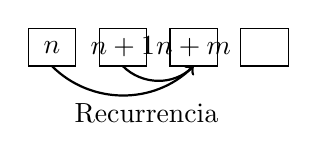
\begin{tikzpicture}[scale=0.6]
            % Diagrama del proceso de recurrencia
            \foreach \i/\label in {0/n,1/{n+1},2/{n+m},3/{}} {
                \draw (\i*1.5,0) rectangle (\i*1.5+1,0.8);
                \node at (\i*1.5+0.5,0.4) {$\label$};
            }
            
            \draw[->, thick] (0.5,0) to[out=-45, in=-135] (3.5,0);
            \draw[->, thick] (2,0) to[out=-45, in=-135] (3.5,0);
            
            \node at (2.5,-1) {Recurrencia};
        \end{tikzpicture}
    \end{columns}
    
    \begin{exampleblock}{Pseudocódigo simplificado}
        1. Inicializar vector de estado con semilla\\
        2. Para cada número generado:\\
        \hspace*{1cm} a. Actualizar parte del vector de estado con recurrencia\\
        \hspace*{1cm} b. Aplicar transformación "tempering" al valor extraído\\
        \hspace*{1cm} c. Retornar el valor normalizado
    \end{exampleblock}
\end{frame}

\begin{frame}{Comparación con generadores integrados en R y Python}
    \begin{lstlisting}[language=R]
# Uso del generador Mersenne Twister en R
set.seed(12345)  # Establecer semilla para reproducibilidad
r_random <- runif(1000)  # Genera 1000 números aleatorios U(0,1)

# Análisis básico
summary(r_random)
    \end{lstlisting}

    \begin{lstlisting}[language=Python]
import numpy as np
import matplotlib.pyplot as plt

# Uso del generador Mersenne Twister en Python
np.random.seed(12345)  # Establecer semilla para reproducibilidad
py_random = np.random.random(1000)  # 1000 números aleatorios U(0,1)

# Análisis básico
print(np.mean(py_random))
print(np.std(py_random))
    \end{lstlisting}
\end{frame}

\section{Pruebas de Aleatoriedad}

\begin{frame}{¿Cómo evaluar la calidad de los generadores?}
    \begin{block}{Pruebas estadísticas de aleatoriedad}
        \begin{itemize}
            \item \textbf{Pruebas de frecuencia}: ¿Están uniformemente distribuidos?
            \item \textbf{Pruebas de series}: ¿Hay patrones en pares o tripletas sucesivas?
            \item \textbf{Pruebas de rachas}: ¿Las rachas son del tamaño esperado?
            \item \textbf{Pruebas espectrales}: Análisis en el dominio de la frecuencia
            \item \textbf{Baterías de pruebas}: DieHard, TestU01, NIST
        \end{itemize}
    \end{block}
    
    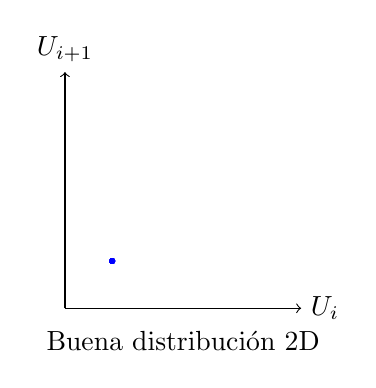
\begin{tikzpicture}[scale=0.6]
        % Visualización de distribución de puntos
        \draw[->] (0,0) -- (5,0) node[right] {$U_i$};
        \draw[->] (0,0) -- (0,5) node[above] {$U_{i+1}$};
        
        % Puntos de un buen generador
        \foreach \i in {1,...,50} {
            \pgfmathsetmacro{\x}{5*rand()}
            \pgfmathsetmacro{\y}{5*rand()}
            \fill[blue] (\x,\y) circle (0.06);
        }
        
        \node at (2.5,-0.7) {Buena distribución 2D};
    \end{tikzpicture}
\end{frame}

\begin{frame}{Prueba de Chi-cuadrado para uniformidad}
    \begin{block}{Procedimiento}
        1. Dividir el intervalo [0,1) en $k$ subintervalos iguales
        2. Contar las frecuencias observadas en cada subintervalo ($O_i$)
        3. Calcular la frecuencia esperada para distribución uniforme ($E_i = n/k$)
        4. Calcular el estadístico:
        \begin{align}
        \chi^2 = \sum_{i=1}^{k} \frac{(O_i - E_i)^2}{E_i}
        \end{align}
        5. Comparar con el valor crítico de $\chi^2_{k-1,\alpha}$
    \end{block}
\end{frame}

\begin{frame}{Implementación de prueba Chi-cuadrado en R}
    \begin{lstlisting}[language=R]
# Función para realizar prueba chi-cuadrado de uniformidad
test_uniformidad <- function(numeros, bins=10) {
  # Contar frecuencias
  frecuencias <- table(cut(numeros, breaks=bins))
  
  # Calcular chi-cuadrado
  n <- length(numeros)
  esperados <- n/bins
  chi_sq <- sum((frecuencias - esperados)^2 / esperados)
  
  # Grados de libertad
  gl <- bins - 1
  
  # p-valor
  pval <- 1 - pchisq(chi_sq, df=gl)
  
  # Resultado
  return(list(
    chi_cuadrado = chi_sq,
    grados_libertad = gl,
    p_valor = pval,
    rechazar_H0 = pval < 0.05
  ))
}

# Generar números con el generador de R
set.seed(42)
nums_r <- runif(1000)

# Aplicar prueba
resultados <- test_uniformidad(nums_r)
print(resultados)
    \end{lstlisting}
\end{frame}

\begin{frame}{Prueba de rachas (runs test)}
    \begin{exampleblock}{¿Qué son las rachas?}
        Una racha es una secuencia de valores consecutivos que están por encima o por debajo de la mediana.
    \end{exampleblock}
    
    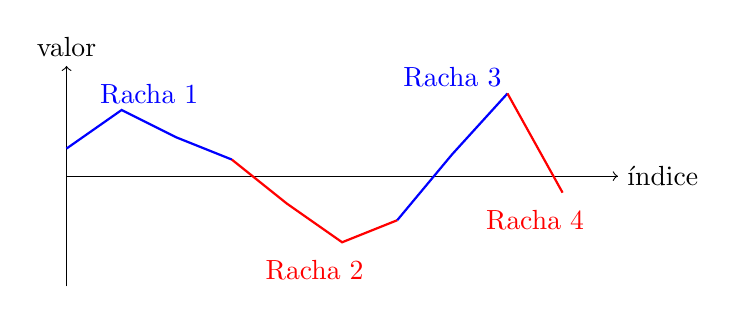
\begin{tikzpicture}[scale=0.7]
        % Visualizar rachas
        \draw[->] (0,0) -- (10,0) node[right] {índice};
        \draw[->] (0,-2) -- (0,2) node[above] {valor};
        \draw[dashed] (0,0) -- (10,0);
        
        \draw[thick, blue] (0,0.5) -- (1,1.2) -- (2,0.7) -- (3,0.3);
        \draw[thick, red] (3,0.3) -- (4,-0.5) -- (5,-1.2) -- (6,-0.8);
        \draw[thick, blue] (6,-0.8) -- (7,0.4) -- (8,1.5);
        \draw[thick, red] (8,1.5) -- (9,-0.3);
        
        \node[blue] at (1.5,1.5) {Racha 1};
        \node[red] at (4.5,-1.7) {Racha 2};
        \node[blue] at (7,1.8) {Racha 3};
        \node[red] at (8.5,-0.8) {Racha 4};
    \end{tikzpicture}
\end{frame}

\begin{frame}{Implementación de prueba de rachas en Python}
    \begin{lstlisting}[language=Python]
import numpy as np
from statsmodels.stats.diagnostic import runstest_1samp

# Generar números aleatorios
np.random.seed(42)
nums = np.random.random(1000)

# Aplicar prueba de rachas
median = np.median(nums)
runs, runs_pval, runs_above, runs_below = runstest_1samp(
    nums, cutoff=median)

print(f"Estadístico de prueba: {runs}")
print(f"p-valor: {runs_pval}")
print(f"Rachas por encima de la mediana: {runs_above}")
print(f"Rachas por debajo de la mediana: {runs_below}")

# Interpretar resultado
alpha = 0.05
if runs_pval < alpha:
    print("Rechazamos H0: Los datos no son independientes")
else:
    print("No rechazamos H0: Los datos parecen independientes")
    \end{lstlisting}
\end{frame}

\section{Aplicación Práctica}

\begin{frame}{Caso de estudio: Simulación de Monte Carlo}
    \begin{block}{Estimación del valor de $\pi$ usando números aleatorios}
        1. Generar puntos aleatorios $(x,y)$ en el cuadrado $[-1,1] \times [-1,1]$
        2. Contar cuántos puntos caen dentro del círculo de radio 1
        3. Estimar $\pi$ como: $\pi \approx 4 \times \frac{\text{puntos dentro del círculo}}{\text{total de puntos}}$
    \end{block}
    
    \begin{tikzpicture}[scale=1.5]
        % Dibujar cuadrado y círculo
        \draw[thick] (-1,-1) rectangle (1,1);
        \draw[thick] (0,0) circle (1);
        
        % Generar puntos aleatorios
        \foreach \i in {1,...,100} {
            \pgfmathsetmacro{\x}{2*rand()-1}
            \pgfmathsetmacro{\y}{2*rand()-1}
            \pgfmathsetmacro{\inside}{ifthenelse(\x*\x+\y*\y<=1, 1, 0)}
            \ifnum\inside=1
                \fill[blue] (\x,\y) circle (0.02);
            \else
                \fill[red] (\x,\y) circle (0.02);
            \fi
        }
        
        % Etiquetas
        \node at (0,-1.3) {Aproximación de $\pi$ por Monte Carlo};
    \end{tikzpicture}
\end{frame}

\begin{frame}{Implementación de la estimación de $\pi$ en R}
    \begin{lstlisting}[language=R]
# Estimar pi usando método de Monte Carlo
estimar_pi <- function(n, generador = "mt") {
  if (generador == "mt") {
    set.seed(42)
    x <- runif(n, -1, 1)
    y <- runif(n, -1, 1)
  } else if (generador == "lcg") {
    # Usar nuestro generador LCG
    seed <- 12345
    x <- lcg(n, seed) * 2 - 1
    y <- lcg(n, seed + 1) * 2 - 1
  }
  
  # Contar puntos dentro del círculo
  dentro <- sum(x^2 + y^2 <= 1)
  
  # Estimar pi
  pi_estimado <- 4 * dentro / n
  
  return(pi_estimado)
}

# Comparar resultados con diferentes tamaños de muestra
tamaños <- c(100, 1000, 10000, 100000)
resultados <- sapply(tamaños, estimar_pi)

# Mostrar resultados
data.frame(Tamaño = tamaños, Pi_estimado = resultados, 
           Error = abs(resultados - pi))
    \end{lstlisting}
\end{frame}

\begin{frame}{Resultados comparativos entre generadores}
    \begin{columns}
        \column{0.5\textwidth}
        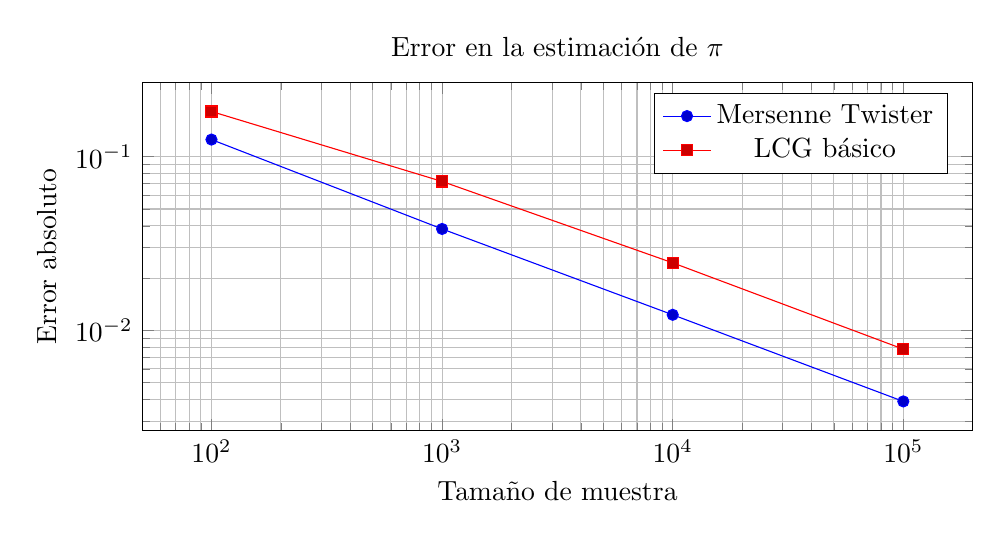
\begin{tikzpicture}
            \begin{axis}[
                width=\textwidth,
                height=6cm,
                title={Error en la estimación de $\pi$},
                xlabel={Tamaño de muestra},
                ylabel={Error absoluto},
                xmode=log,
                ymode=log,
                log basis x=10,
                legend pos=north east,
                grid=both
            ]
            
            % Datos simulados 
            \addplot coordinates {
                (100, 0.1256)
                (1000, 0.0384)
                (10000, 0.0123)
                (100000, 0.0039)
            };
            \addlegendentry{Mersenne Twister}
            
            \addplot coordinates {
                (100, 0.1823)
                (1000, 0.0721)
                (10000, 0.0245)
                (100000, 0.0078)
            };
            \addlegendentry{LCG básico}
            
            \end{axis}
        \end{tikzpicture}

        \column{0.5\textwidth}
        \begin{alertblock}{Observaciones}
            \begin{itemize}
                \item El error disminuye aproximadamente como $\frac{1}{\sqrt{n}}$
                \item Mersenne Twister produce estimaciones más precisas
                \item LCG muestra mayor variabilidad
                \item Para aplicaciones críticas, se recomienda MT
            \end{itemize}
        \end{alertblock}
    \end{columns}
\end{frame}

\section{Ejercicios Propuestos}

\begin{frame}{Ejercicios propuestos}
    \begin{enumerate}
        \item Implementar un generador congruencial lineal con parámetros $a=69069$, $c=1$ y $m=2^{32}$. Realizar una prueba de chi-cuadrado para verificar la uniformidad de los números generados.
        
        \item Generar 1000 pares de números aleatorios $(U_i, U_{i+1})$ usando el generador de R/Python y visualizarlos en un diagrama de dispersión. ¿Observa algún patrón? Repetir el ejercicio con un LCG simple y comparar.
        
        \item Implementar una prueba de autocorrelación para verificar la independencia de los números generados. Aplicarla a secuencias generadas con diferentes generadores y comparar los resultados.
    \end{enumerate}
\end{frame}

\section{Referencias Bibliográficas}

\begin{frame}{Referencias bibliográficas}
    \begin{itemize}
        \item Gentle, J.E. (2009). Computational Statistics. Springer. Capítulo 5.
        
        \item L'Ecuyer, P. (1999). Good parameters and implementations for combined multiple recursive random number generators. \textit{Operations Research}, 47(1), 159-164.
        
        \item Matsumoto, M., \& Nishimura, T. (1998). Mersenne twister: a 623-dimensionally equidistributed uniform pseudo-random number generator. \textit{ACM Transactions on Modeling and Computer Simulation}, 8(1), 3-30.
        
        \item Knuth, D. (1997). The Art of Computer Programming, Volume 2: Seminumerical Algorithms. Addison-Wesley.
        
        \item L'Ecuyer, P., \& Simard, R. (2007). TestU01: A C library for empirical testing of random number generators. \textit{ACM Transactions on Mathematical Software}, 33(4), 22.
    \end{itemize}
\end{frame}

\begin{frame}{Actividad práctica}
    \begin{exampleblock}{Actividad: Comparación empírica de generadores}
        Trabajando en grupos de 2-3 personas:
        \begin{enumerate}
            \item Implementar dos generadores diferentes de números aleatorios:
            \begin{itemize}
                \item Un LCG con parámetros a elección
                \item Usar el generador integrado en R/Python
            \end{itemize}
            \item Para cada generador:
            \begin{itemize}
                \item Realizar al menos 2 pruebas estadísticas de aleatoriedad
                \item Generar visualizaciones para comparar la calidad
                \item Utilizar ambos en la estimación de $\pi$ y comparar resultados
            \end{itemize}
            \item Preparar un breve reporte con conclusiones
        \end{enumerate}
        
        \textbf{Fecha de entrega:} Próxima sesión
    \end{exampleblock}
\end{frame}

\begin{frame}{Próxima sesión}
    \begin{block}{Sesión 5: Generación de Variables Aleatorias}
        \begin{itemize}
            \item Método de la transformación inversa
            \item Método de aceptación-rechazo
            \item Método de composición
            \item Implementación en R y Python
        \end{itemize}
    \end{block}
    
    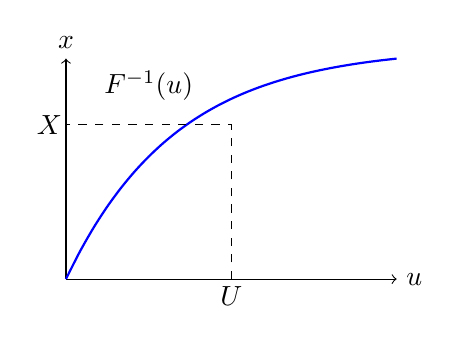
\begin{tikzpicture}[scale=0.7]
        % Visualización de la transformación inversa
        \draw[->] (0,0) -- (6,0) node[right] {$u$};
        \draw[->] (0,0) -- (0,4) node[above] {$x$};
        
        % Función CDF y su inversa
        \draw[domain=0:1, smooth, variable=\x, blue, thick] 
            plot ({6*\x}, {4*(1-(exp(-3*\x)-exp(-3))/(1-exp(-3)))});
        
        \draw[dashed] (3,0) -- (3,2.8) -- (0,2.8);
        
        \node at (3,-0.3) {$U$};
        \node at (-0.3,2.8) {$X$};
        \node at (1.5,3.5) {$F^{-1}(u)$};
    \end{tikzpicture}
\end{frame}

\end{document}
